Excluding the E layer cells that are connected only to one PMT, the cell noise
is the combination of the two readout channels of a cell where the digital noise
from the PMTs is added quadratically and converted in MeV using the calibration
constants and \cref{eq:84}. There are four possible gain combinations:
\gls{hghg}, \gls{lglg}, \gls{lghg} and \gls{hglg}. When the energy deposit is
large, the two channels belonging to the cell are readout in low gain thus
giving rise to the LGLG combination, for small signals the HGHG combination is
used. It can also occur that for energy deposits in the intermediate range, one
PMT is readout in LG and the other in HG resulting in a HGLG combination. The
cell noise is used to identify the seed cells in the topocluster algorithm (see
Section~\ref{sec:topocluster}).

Figure~\ref{fig:non_gaussianity} shows a comparison between the cell noise and
the fitted $\sigma$ parameter of a normal distribution. The ratio RMS / $\sigma$
= 1 indicates a perfect agreement between the measured and the fitted amplitude
distribution for a single Gaussian hypothesis. The blue square in the plot
indicate the comparison for an old model of \gls{lvps} while the red square
refers to the currently used LVPSs. It can be seen that with the old model of
\glspl{lvps} the ratio RMS / $\sigma$ can be large indicating a non Gaussian
behavior of the electronic noise. For this reason a double Gaussian distribution
is used to fit the energy distribution with the probability density function
defined as:
\begin{equation}
  \label{eq:85}
  f_{2g} = \frac{1}{1 + R} \left( \frac{1}{\sqrt{2 \pi} \sigma_1} e^{-
      \frac{x^2}{2 \sigma_1^2}} + \frac{R}{\sqrt{2 \pi} \sigma_2} e^{-
      \frac{x^2}{2 \sigma_2^2}} \right)
\end{equation}
where $R$ is the relative normalization of the two Gaussians and
$\sigma_1, \sigma_2$ and $R$ are independent parameters. These three are used to
define the region $\sigma_{\text{eff}}(E)$ where the significance for the double
Gaussian is the same as the one $\sigma$ region for a single Gaussian,
i.e.
$\int_{- \sigma_{\text{eff}}}^{\sigma_{\text{eff}}} f_{2g} =
0.68$~\cite{TileReadiness}.
In terms of $\sigma_{\text{eff}}$, for an energy deposit $E$, the significance
can be expressed as:
\begin{equation}
  \label{eq:86}
  \frac{E}{\sigma_{\text{eff}}(E)} = \sqrt{2}\ \text{Erf}^{- 1} \left( \frac{\sigma_1
      \text{Erf} \left(\frac{E}{\sqrt{2 \sigma_1}} \right) + R \sigma_2 \text{Erf}
    \left( \frac{E}{\sqrt{2 \sigma_2}} \right)}{\sigma_1 + R \sigma_2} \right)
\end{equation}
where Erf is the error function. Equation~\ref{eq:86} is the input to the
calorimeter cell clustering algorithm discussed in more details in
\cref{sec:topocluster}, moreover this definition allows to use the same unit to
describe the noise for both the TileCal and LAr calorimeters. The region
$\sigma_{\text{eff}}(E)$ is commonly referred to as \emph{cell noise} and
together with the three double Gaussian parameters ($\sigma_1$, $\sigma_2$ and
R) is stored in the COOL database.

\begin{figure}[!h]
  \centering
    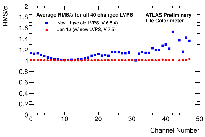
\includegraphics[width=.8\linewidth]{non_gaussianity}
    \caption{Comparison between the TileCal electronic noise, measured as the
      RMS of the reconstructed amplitude distribution in pedestal runs and the
      $\sigma$ of the Gaussian fit of the distribution for the old and new
      LVPS~\cite{TileCalNoisePub}.}
    \label{fig:non_gaussianity}
\end{figure}
%%% Local Variables:
%%% mode: latex
%%% TeX-master: "../search_for_DM_LED_with_ATLAS"
%%% End:
